\documentclass[10pt,aspectratio=43,serif]{beamer}
\usetheme{Berlin}
% \usetheme{Copenhagen}
% 设置为 Beamer 文档类型,设置字体为 10pt,长宽比为4:3(16:9),字体为 serif 风格
\usepackage[UTF8]{ctex}
\usepackage{setspace}
\usepackage{graphicx}
\usepackage{subfigure}
\usepackage{listings}
\lstset{
    basicstyle=\ttfamily,
    language=C++,
    keywordstyle=\bfseries\color{blue!90!black},
    stringstyle=\bfseries\color{green!70!black},
    columns=flexible,
}

\setlength{\parskip}{1em}

\title{Solosis}
\subtitle{基于 LeNet-5 的手写数字识别}

\author{李明翰}
\institute{数学与统计学院 2201 班, 华中科技大学}
\date{\today}
  
\begin{document}

\begin{frame}
    \titlepage
\end{frame} %生成标题页

\section{目录}
\begin{frame}
    \frametitle{目录}
    \tableofcontents
\end{frame}

\section{项目简介}
\begin{frame}
    \frametitle{项目简介}
    \begin{block}{简介}
        用 C++ 实现用于识别手写数字的 LeNet-5 卷积神经网络,采用 MNIST 作为训练集和测试集进行训练,并使用 OpenCV 进行图像支持。        
    \end{block}
    
    \begin{block}{输入}
        一张图片,内容为一张写有黑色数字的白纸。
    \end{block}
    \begin{block}{输出}
        识别后的图片。
    \end{block}
\end{frame}

\begin{frame}
    \frametitle{效果}
    \begin{figure}
        \subfigure[样例输入]{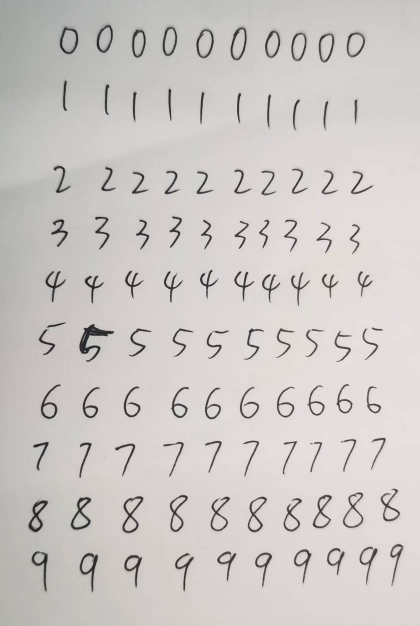
\includegraphics[scale=0.2]{res/sample-input.jpg}}
        \qquad
        \subfigure[样例输出]{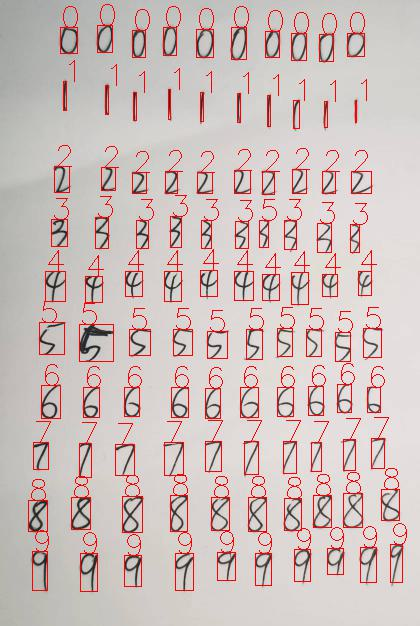
\includegraphics[scale=0.2]{res/sample-output.jpg}}
        \caption{一组样例输入输出}
    \end{figure}
\end{frame}

\section{原理概述}
\subsection{LeNet-5 模型概述}
\begin{frame}
    \frametitle{LeNet-5 模型概述}
    \begin{block}{简介}
        LeNet-5 是一个卷积神经网络模型,可判断一个 $32 \times 32$ 大小的灰度图上所写的数字为 $0 \sim 9$ 中的哪一个。
    \end{block}
    
    \begin{block}{输入}
        一个 $32 \times 32$ 的矩阵 $\mathbf A$,其中 $A_{i, j} \in [0, 1]$ 表示第 $i$ 行第 $j$ 列的像素点的亮度。
    \end{block}
    
    \begin{block}{输出}
        一个整数 $y \in [0, 9]$,表示其预测的数字。
    \end{block}
\end{frame}

\begin{frame}
    \frametitle{LeNet-5 模型概述}
    \begin{alertblock}{警告}
        由篇幅所限,模型结构、训练算法等均不展开阐述,不建议没有基础的同学学习这一部分。
        
        本项目提供了已经训练过的模型和各种函数,可以直接使用。
    \end{alertblock}
\end{frame}

\subsection{对单个数字进行分类}
\begin{frame}
    \frametitle{对单个数字进行分类}
    \begin{enumerate}
        \item 灰度化
        \item 亮度离差标准化至 $[0, 255]$
        \item 阈值修改
        \item 检测图形的边框并裁剪
        \item 放缩为 $32 \times 32$ 大小
        \item 再次亮度离差标准化
        \item 将其作为输入提供给 LeNet-5 模型,得到输出
    \end{enumerate}
\end{frame}

\begin{frame}
    \frametitle{灰度化}
    即将彩色图片变为灰色图片。
    
    如果需要,将图片反色,使得图片为黑底白字。
    
    \begin{figure}
        \subfigure[处理前]{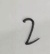
\includegraphics[scale=0.8]{res/d0.jpg}}
        \qquad
        \subfigure[处理后]{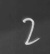
\includegraphics[scale=0.8]{res/d1.jpg}}
    \end{figure}
\end{frame}

\begin{frame}
    \frametitle{亮度离差标准化}
    记最小、最大亮度分别为 $\min, \max$,定义 $\text{round}(x)$ 表示 $x$ 四舍五入得到的整数。若 $\min \neq \max$,则对像素点 $A_{i, j}$,改变其亮度为
    
    $$\text{round}(\frac {A_{i, j} - \min}{\max - \min} \times 255)$$
    
    也就是将 $[\min, \max]$ 线性映射到 $[0, 255]$,避免亮度不统一的情况。
    
    \begin{figure}
        \subfigure[处理前]{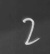
\includegraphics[scale=0.8]{res/d1.jpg}}
        \qquad
        \subfigure[处理后]{
\includegraphics[scale=0.8]{res/d2.jpg}}
    \end{figure}
\end{frame}

\begin{frame}
    \frametitle{阈值修改}
    对每个像素点,若亮度小于 $C$($C$ 为常数),将其亮度设置为 $0$。
    
    避免具有微弱亮度的像素点对模型判断的影响。
    
    \begin{exampleblock}{提示}
        本项目中取 $C = 130$。        
    \end{exampleblock}
    
    \begin{figure}
        \subfigure[处理前]{
\includegraphics[scale=0.8]{res/d2.jpg}}
        \qquad
        \subfigure[处理后]{
\includegraphics[scale=0.8]{res/d3.jpg}}
    \end{figure}
\end{frame}

\begin{frame}
    \frametitle{检测图形的边框并裁剪}
    边框:最小的、能包含所有亮度非 $0$ 的像素点的矩形。
    
    检测边框,裁剪出子图。
    
    避免书写位置的影响。
    
    \begin{figure}
        \subfigure[处理前]{
\includegraphics[scale=0.8]{res/d3.jpg}}
        \qquad
        \subfigure[处理后]{
\includegraphics[scale=0.8]{res/d4.jpg}}
    \end{figure}
\end{frame}

\begin{frame}
    \frametitle{放缩为 $32 \times 32$ 大小}
    避免书写大小不同的影响。
    
    \begin{exampleblock}{提示}
        此处放缩为非比例放缩。
        
        尽管强制放缩得到的图片可能很奇怪(如数字 $1$ 放缩后可能是一张几乎全亮的图片),但只需要保证多张同一数字的图片,经过放缩后得到的图片相近即可。
    \end{exampleblock}
    
    \begin{figure}
        \subfigure[处理前]{
\includegraphics[scale=0.8]{res/d4.jpg}}
        \qquad
        \subfigure[处理后]{
\includegraphics[scale=0.8]{res/d5.jpg}}
    \end{figure}
\end{frame}

\begin{frame}
    \frametitle{再次亮度离差标准化}
    避免放缩后导致亮度变暗的情况。
    
    \begin{figure}
        \subfigure[处理前]{
\includegraphics[scale=0.8]{res/d5.jpg}}
        \qquad
        \subfigure[处理后]{
\includegraphics[scale=0.8]{res/d6.jpg}}
    \end{figure}
\end{frame}

\subsection{对整张图片进行分类}
\begin{frame}
    \frametitle{对整张图片进行分类}
    
    \begin{block}{预处理}
        先灰度化,然后进行阈值修改。
    \end{block}
    
    \begin{block}{判断边界}
        对每一个有亮度的点进行深度优先搜索,搜索出整个联通块,提供给 LeNet-5 作为单张图片进行判断。
        
        其中点 $(i, j)$ 和点 $(x, y)$ 联通,当且仅当两个点的亮度非 $0$ 且 $\max\{|i - x|, |j - y|\} \leq D$,其中 $D$ 为常数。
    \end{block}
    
    \begin{exampleblock}{提示}
        本项目中取 $D = 6$。
    \end{exampleblock}
\end{frame}


\section{项目结构}
\subsection{项目结构概述}
\begin{frame}
    \frametitle{项目结构概述}
    项目根目录文件夹 \texttt{solosis} 下共有:

    \begin{itemize}
        \item 文件夹 \texttt{doc}:储存说明文档。
        \item 文件夹 \texttt{include}:储存 C++ \texttt{.h} 头文件。
        \item 文件夹 \texttt{mnist-data}:储存用于训练的 MNIST 数据。
        \item 文件夹 \texttt{model-data}:储存模型数据。
        \item 文件夹 \texttt{source}:储存 C++ \texttt{.cpp} 源代码。
        \item 文件 \texttt{.clang-format}:clang-format 格式化配置文件。
        \item 文件 \texttt{main.cpp}:C++ 主程序。
        \item 文件 \texttt{makefile}:指定编译方式的 Makefile。
    \end{itemize}
\end{frame}

\subsection{LeNet-5 使用方法}
\begin{frame}
    \frametitle{LeNet-5 使用方法}
    \texttt{include/lenet.h} 提供了一个名为 \lstinline|Lenet| 的类,拥有已经封装好的接口,可以直接调用。

    \begin{block}{初始化}
        \lstinline|Lenet::Lenet(const char *filepath)|:从 \lstinline|filepath| 读入模型参数。
    \end{block}

    \begin{block}{使用}
        \lstinline|int Lenet::predict(float in[32][32])|:将 \lstinline|in| 作为输入,返回模型预估的数字。
        
        其中 \lstinline|in[i][j]| 应当为 $[0, 1]$ 间的实数,背景色为 $0$,字迹色为 $1$。
    \end{block}
\end{frame}

\begin{frame}[fragile]
    \frametitle{LeNet-5 使用样例}
\begin{lstlisting}
#include "lenet.h"
#include <iostream>
#include <opencv2/opencv.hpp>
using namespace cv;
using namespace std;
int main() {
    Lenet lenet = Lenet("model-data/standard.model");
    Mat image = imread("test-digit.jpg");
    float in[32][32];
    for (int i = 0; i < 32; i++)
        for (int j = 0; j < 32; j++)
            in[i][j] = image.at<uchar>(i, j) / 255.0;
    cout << lenet.predict(in) << endl;
    return 0;
}
\end{lstlisting}
\end{frame}

\end{document}
